    \textbf{Four Degrees of Separation}
    
    The pioneering work of the sociologist Stanley Milgram led to what is now termed the \textit{small world phenomenon}, the idea that any two people on the earth are reachable within at most six steps. When considering connected subsets of people, we can get this down to a smaller number - indeed, in the paper \textit{Four Degrees of Separation} (Backstrom, Boldi, et al)\footnote{http://arxiv.org/abs/1111.4570}, the authors show that, as of January 2012, Facebook has 4.74 degrees of separation between any two active users. The paper can be split into two sections. The first, which we shall discuss only briefly, deals with the technological challenges of analysing subgraphs of the Facebook network. The second deals with the mathematics of networks and network theory; it is the main focus of this essay.
    
    The authors use an algorithm called \textit{layered labelled propagation}\footnote{introduced by Boldi, Rosa, et. al in \href{https://arxiv.org/pdf/1011.5425.pdf}{their paper} the year prior.} to compress the network. LLP achieves a high level of compression for a localised, similar network. The Facebook network achieves 30\% compression under LLP; the network is seen to be highly localised and similar. 
    
    \begin{figure}[H]
        \centering
        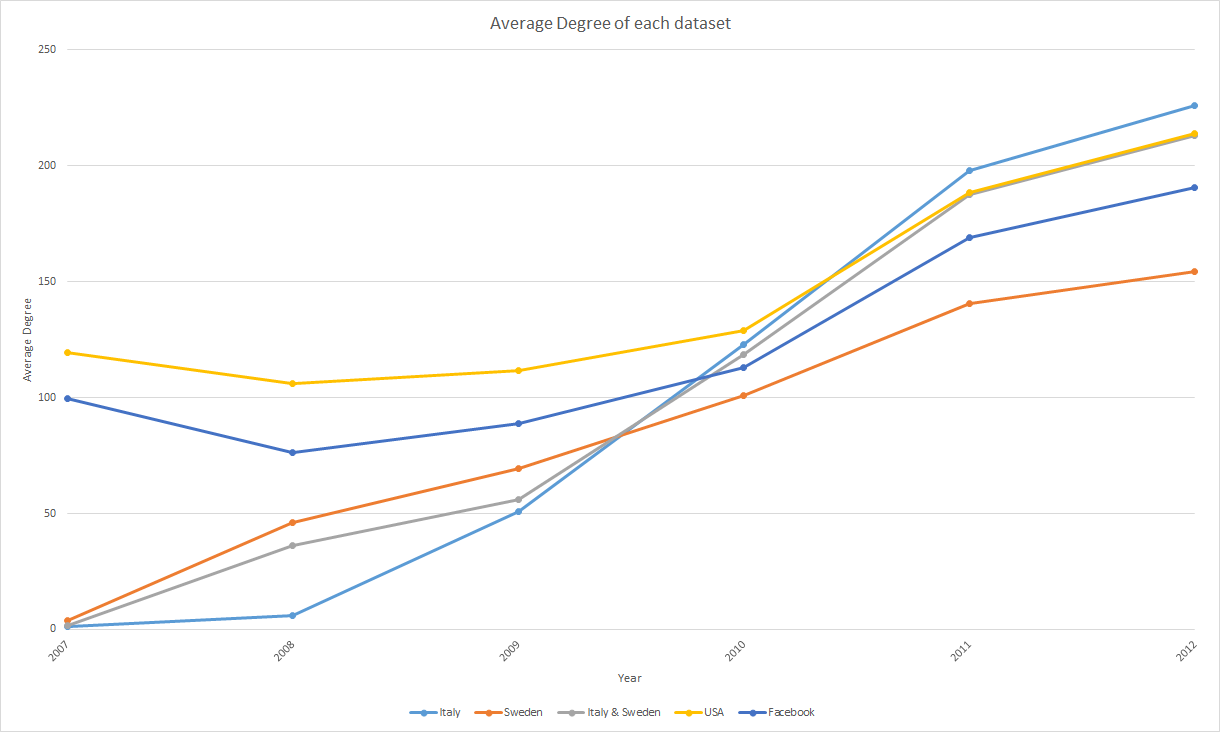
\includegraphics[width=\textwidth]{SR-AverageDegree.png}
        \caption{Average Degree of each subgraph}
        \label{fig:avdeg}
    \end{figure}
    \begin{table}[H]
        \centering
        \begin{tabular}{c|c|c|c|c|c}
            \toprule
            & Italy & Sweden & Italy $\cup$ Sweden & USA & Facebook \\
            \midrule
            2007 & 1.31 & 3.90 & 1.50 & 119.61 & 99.5 \\
            2008 & 5.88 & 46.09 & 36.00 & 106.05 & 76.15 \\
            2009 & 50.82 & 69.60 & 55.91 & 111.78 & 88.68 \\
            2010 & 122.92 & 100.85 & 118.54 & 128.95 & 113.00 \\
            2011 & 198.20 & 140.55 & 187.48 & 188.30 & 169.03 \\
            2012 & 226.03 & 154.54 & 213.30 & 213.76 & 190.44 \\
            \bottomrule
        \end{tabular}
        \caption{Average Degree of each subgraph}
        \label{tab:avdeg}
    \end{table}
    
    Interesting comparisons can be drawn from this data about the virality of Facebook in markets outside of the United States; given that it took Italian users until 2010 to reach the average degree that the USA had in 2007, we can say with confidence that Facebook did not catch on in Italy until much later on in Facebook's existence. With the number of active Facebook users now exceeding 2.4 billion (when this paper was published it was 0.724 billion), there would be some interesting data if one could extract historical records.\footnote{In order to preserve user anonymity and respect laws like GDPR in Europe, Facebook tends not to retain much historical information} Given that a non-negligible portion of the global population is on Facebook, given access to the full user network we could examine whether the theory of six degrees (or even four) of separation is true.
    
    \begin{figure}[H]
        \centering
        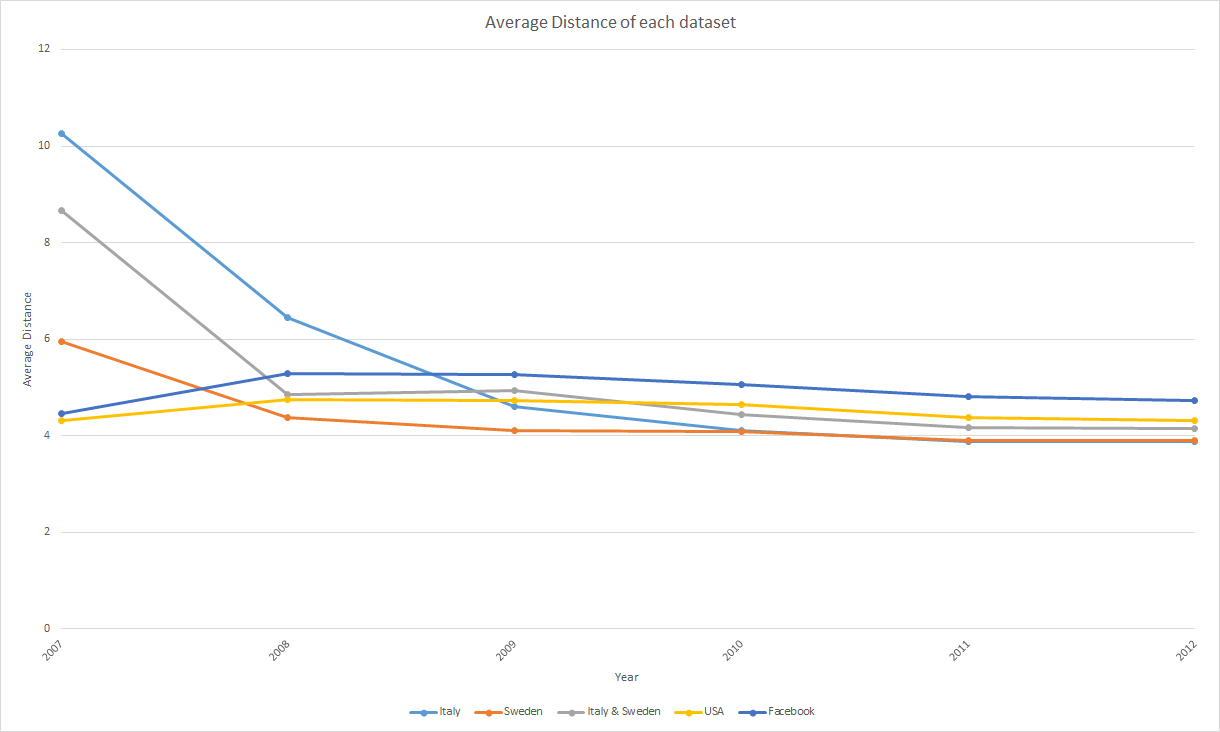
\includegraphics[width=\textwidth]{SR-AverageDistance}
        \caption{Average distance for each dataset. Note that the distance for the Facebook set in 2012 is 4.74.}
        \label{fig:avdist}
    \end{figure}
    
    We see that the average distance of all the subnetworks tends towards a central value as they all grow in size. That value for Facebook is approximately 4.74 in the year 2012. This is what we expect of a scale-free network, which this network appears to be - considering one component of the graph is analogous to considering the graph as a whole, similar to ergodic processes in Thermodynamics. Moreover, as the network continues to grow (whether that be through artificial growth or by considering larger and larger components such as the set Italy $\cup$ Sweden in our examples), we would see the average distance converge to the global value.
    
    Further to this; the authors define the \textit{spid} of a network (or \textit{index of dispersion}) as its variance-to-mean ratio, that is, $s\equiv\frac{\sigma^2}{\mu}$. A proper social network is expected to have $s\ll 1$, whilst a web graph is expected to have $s>1$. The entire paper is motivated as trying to find the spid of Facebook; indeed the authors find that $s_{facebook}=0.09\pm0.003$ for the year 2012. The authors go further, showing that spid is not correlated in general to average distance, as shown in Fig.~\ref{fig:avdistspid} (their Fig. 7).
    
    \begin{figure}[H]
        \begin{minipage}{.5\textwidth}
        The phenomena of small world networks gives rise to scale-free networks. In a scale free network, the network is ergodic. Symbolically, it follows a power law, that is $P_k\propto k^{-\gamma}$ where $\gamma\in\mathbb{R}$. It is known\footnotemark[3] that there are relationships between small-world and scale-free networks, and that networks that can be generated via PAGP algorithms tend to be scale-free\footnotemark[4]. Given that social networks by their very nature are generated with a PAGP model - the so-called \textit{friendship paradox} states that "your friends have more friends than you" - we see that social networks should also obey a power law. Whether they do in practice or not remains an open question.
        \end{minipage}%
        \begin{minipage}{.5\textwidth}\centering
            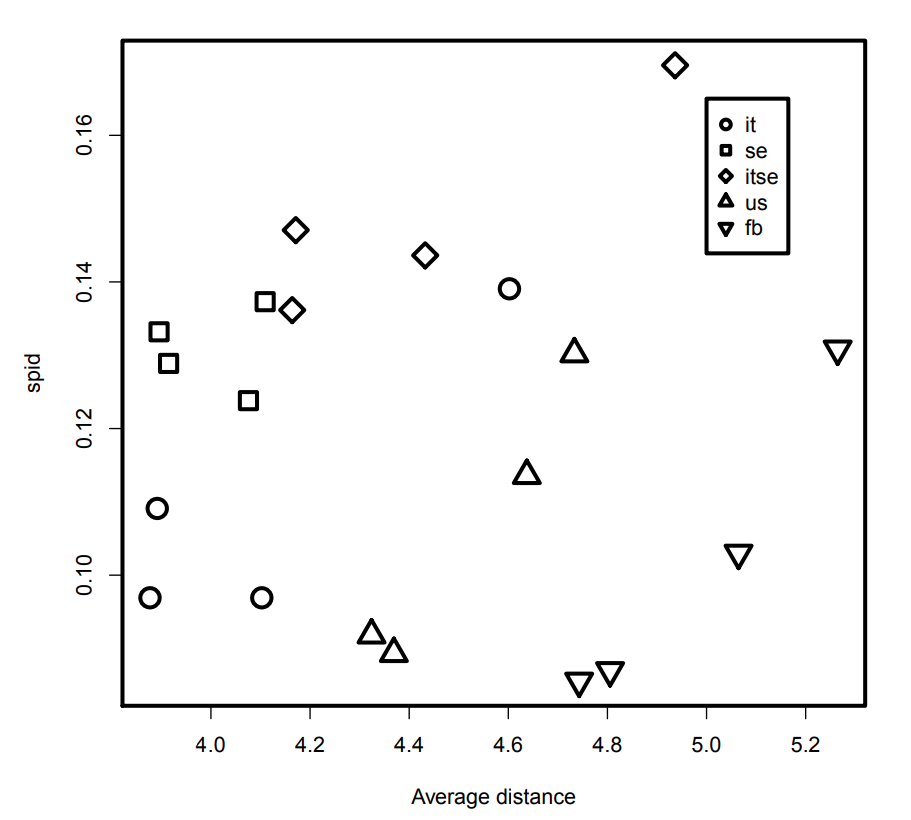
\includegraphics[width=\textwidth]{SR-SpidVsDistance.PNG}
            \caption{Spid vs. Average Distance (Backstrom, Boldi, et al)}
            \label{fig:avdistspid}
        \end{minipage}
    \end{figure}
    
    \footnotetext[3]{https://ieeexplore.ieee.org/document/6505891}
    \footnotetext[4]{ibid}